\chapter{Motivation}
\label{ch:motivation}

Distributed consensus systems have become a critical component of modern internet infrastructure, powering every major internet application at some level or another.

The most common paradigm for studying and implementing distributed consensus is that of the Replicated State Machine, 
wherein a \emph{deterministic} state machine is replicated across a set of nodes, 
such that it functions as a single state machine despite the failure of some nodes.
The state machine is driven by a set of inputs, known as \emph{transactions}, 
where each transaction may or may not, depending on its validity, cause a state transition and return a result.
The state transition logic is governed by the state machine's state transition function,
which maps a transaction and the current state to a new state and a return value.
The state transition function is also sometimes referred to as \emph{application logic}.

It is the responsibility of the consensus protocol to order the transactions so that the resulting 
\emph{transaction log} is replicated exactly on every node.
Using a deterministic state transition function implies that 
every node will compute the same state given the same transaction log.

A summary of the replicated state machine architecture is given in Figure \ref{fig:replicated_state_machine}.

\begin{figure}[]
	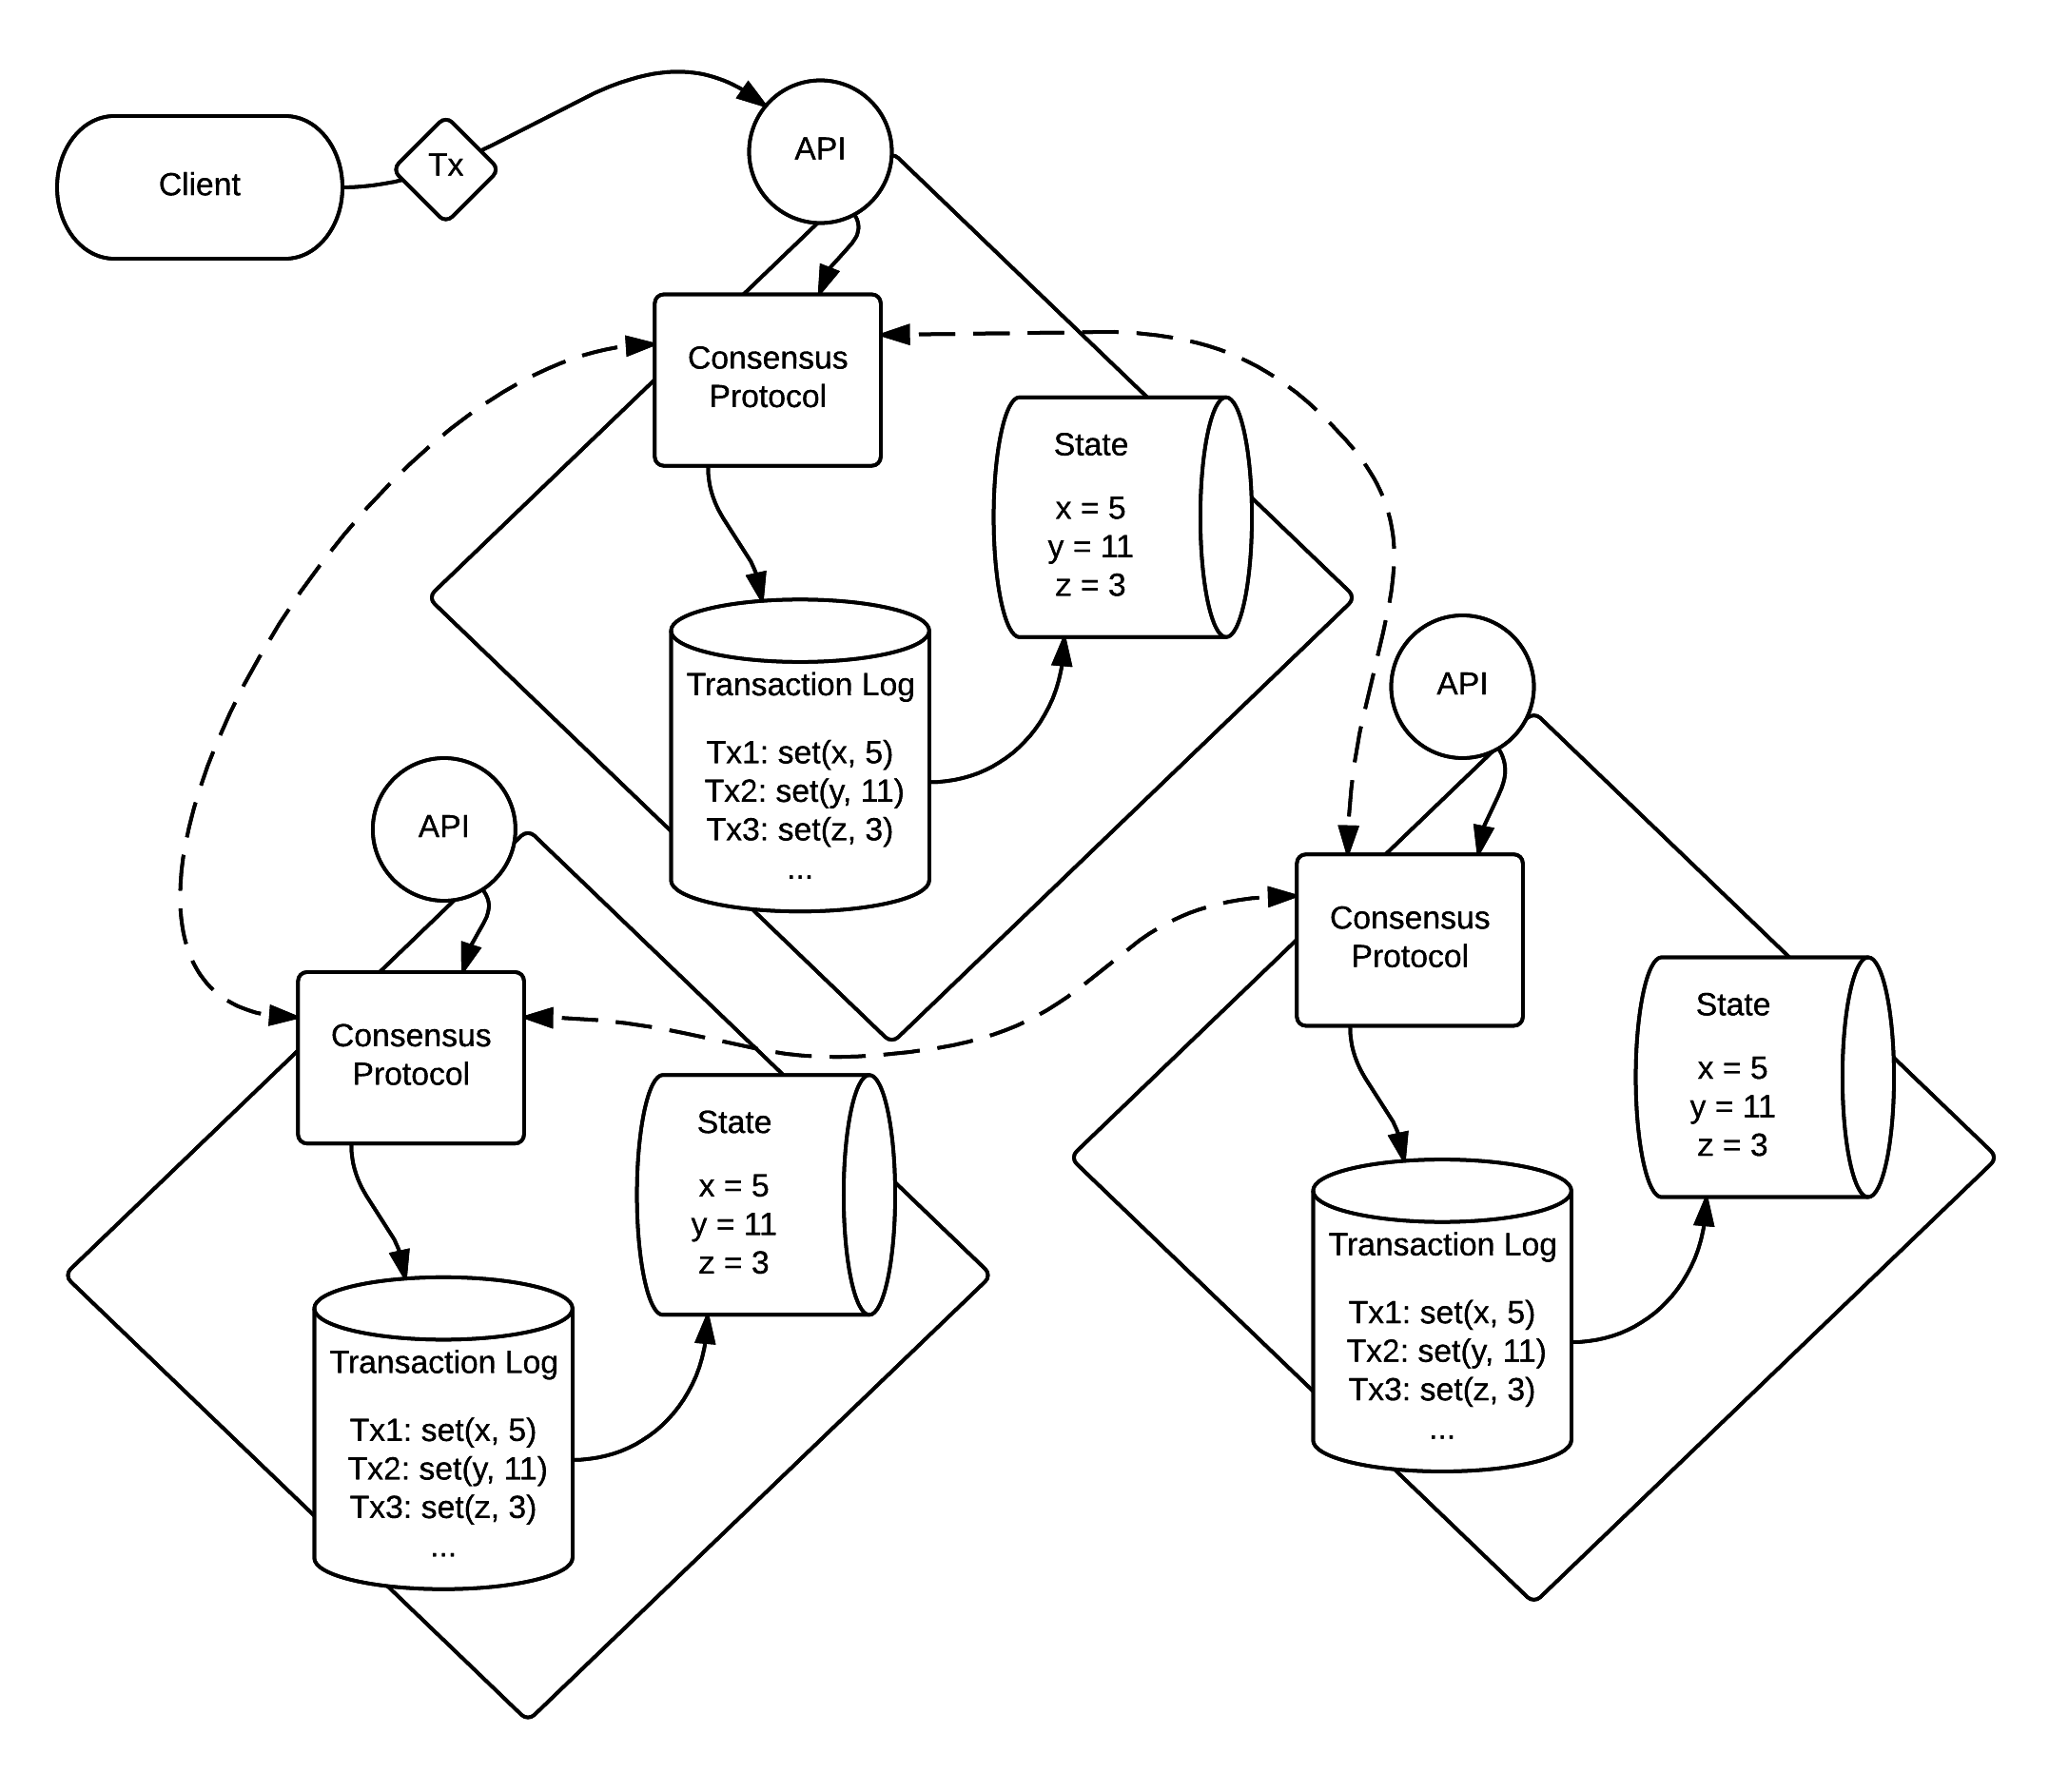
\includegraphics[width=\linewidth,height=\textheight,keepaspectratio]{figures/state_machine.png}
    	\centering
	\label{fig:replicated_state_machine}
	\caption[Overview of replicated state machine architecture]{
A replicated state machine replicates a transaction log and resulting state across multiple machines. 
Transactions are received from the client, 
run through the consensus protocol, 
ordered in the transaction log,
and executed against the state. 
In the figure, each diamond represents a single machine, 
with dotted lines representing communication between machines to carry out the consensus protocol for ordering transactions.}
\end{figure}

Tendermint was motivated from the desire to create a general purpose, high-performance, secure, and robust replicated state machine.

\section{Distributed Consensus}

The purpose of a fault-tolerant distributed consensus system is to co-ordinate a network of computers to 
stay in sync while providing a useful service, despite the presence of faults.
Staying in sync amounts to replicating the transaction log successfully; 
providing a useful service amounts to keeping the state machine available for new transactions.
These aspects of the system are traditionally known as \emph{safety} and \emph{liveness}, respectively.
Colloquially, safety means nothing bad happens; liveness means that something good eventually happens.
A violation of safety implies two or more valid, competing transaction logs.
Violating liveness implies an unresponsive network.

It is trivial to satisfy liveness by accepting all transactions. And it is trivial to satisfy safety by accepting none.
Hence, consensus algorithms can be seen to operate on a spectrum defined by these extremes.
Typically, nodes require some threshold of received information from other nodes before they commit a new transaction.
In synchronous environments, 
where we make assumptions about the maximum delay of network messages or the maximum speed of processor clocks,
 it is easy enough to take turns proposing new transactions, poll for a majority vote, 
and skip a proposer's turn if they don't propose within the bounds of the synchrony assumptions.

In asynchronous environments, where no such assumptions about network delays or processor speeds are warranted,
the trade-off is much more difficult to manage.
In fact, the so called FLP impossibility result demonstrates the 
impossibility of distributed consensus among deterministic asynchronous processes 
if even a single process can crash\footnote{Prior to FLP, the distinction between sync/async was not as prominent.}\cite{flp}.
The proof amounts to showing that, because processes can fail, 
there are valid executions of the protocol in which processes fail at the exact opportune times to prevent consensus.
Hence, we have no guarantee of consensus.

Typically, synchrony in a protocol is reflected by the use of timeouts to manage certain transitions.
In asynchronous environments, where messages can be arbitrarily delayed, relying on synchrony (timeouts) for safety
can lead to a fork in the transaction log.
Relying on synchrony to ensure liveness can cause the consensus to halt, and the service to become unresponsive.
The former case is usually considered more severe, as reconciling conflicting logs can be a daunting or impossible task. 

In the early 90s, Lamport broke new ground with the Paxos algorithm \cite{paxos},
which, while not fully asynchronous,
provided the first provably correct algorithm for distributed consensus in mostly asynchronous environments.
Paxos simultaneously empowered and confused the discipline of consensus science,
on the one hand by providing the first real-world, practical, fault-tolerant consensus algorithm,
and on the other by being so difficult to understand and explain.

Paxos became the staple consensus algorithm for industry, 
upon which the likes of Amazon \cite{dynamo}, Google \cite{chubby}, 
and others would build out highly available global internet services.
The Paxos consensus would sit at the bottom of the application stack, 
providing a consistent interface to resource management and allocation, 
operating at much slower time scales than the highly-available applications facing the users.
However, there has always been an understanding in the field that implementing Paxos is somewhat of a black art,
permeated by tricks for two main things: 
maintaining liveness in the face of asynchrony, and achieving consensus on more than one bit at a time.

Like most consensus algorithms before it, the official Paxos algorithm only achieves consensus on one bit at a time,
and involves an expensive leadership election process for each additional bit. 
Hence a variety of so called Multi-Paxos have been proposed, but no single approach dominates, 
and each implementation diverges in its own unique ways. 
The resulting software ecosystem is clumsy, difficult to navigate, and in some cases overly liable to contain bugs.
Some have worked to more more clearly define these difficulties 
and describe solutions \cite{chandra2007paxos}.

Seeking to remedy this situation, in 2013, Ongaro and Ousterhout published Raft \cite{raft},
an algorithm for consensus in asynchronous environments whose motivating design goal was understandability.
Raft is much simpler to understand than Paxos.
It has seen tremendous adoption in the open source community, 
with implementations in virtually ever major language \cite{raft.github.io},
and use as the backbone in major projects, 
including CoreOs's distributed Linux distribution \cite{coreos_raft} and the open source time-series database InfluxDB \cite{influxdb,hashicorp_raft}.

Raft's major divergent design decisions from Paxos was to focus on the transaction-log first, rather than a single bit,
and to allow a leader to persist in committing transactions until he goes down, 
at which point leadership election can kick in. 
In some ways, this is similar to the approach taken by blockchains, 
though the major advantage of blockchains is the ability to tolerate a different kind of fault.

\section{Byzantine Fault Tolerance}

Blockchains have been described as ``trust machines'' \cite{economist_blockchains} on account of the way they reduce counter party risk through the decentralization of responsibility over a shared database.
Bitcoin, in particular, is noted for its ability to withstand attacks and malicious behaviour by any of the participants. 
Traditionally, consensus protocols tolerant of malicious behaviour were known as Byzantine Fault Tolerant (BFT) consensus protocols.
The term Byzantine was used due to the similarity of the problem to that faced by generals of the Byzantine army attempting to co-ordinate themselves to attack Rome using only messengers,
where one of the generals may be a traitor \cite{lamport1982byzantine}.

In a crash fault, a process simply halts. In a Byzantine fault, it can behave arbitrarily.
Crash faults are easier to handle, as no process can \emph{lie} to another process.
Systems which only tolerate crash faults can operate via simple majority rule, 
and therefore typically tolerate simultaneous failure of up to half of the system.
If the number of failures the system can tolerate is $f$, such systems must have at least $2f+1$ processes.

Byzantine failures are more complicated. In a system of $2f+1$ processes, if $f$ are Byzantine, 
they can co-ordinate to say arbitrary things to the other $f+1$ processes.
For instance, suppose we are trying to agree on the value of a single bit, 
and $f=1$, so we have $N=3$ processes, $A$, $B$, and $C$, where $C$ is Byzantine, as in Figure \ref{fig:byzantine}.
$C$ can tell $A$ that the value is $0$ and tell $B$ that it's $1$. 
If $A$ agrees that its $0$, and $B$ agrees that its $1$, then they will both think they have a majority and commit, 
thereby violating the safety condition.
Hence, the upper bound on faults tolerated by a Byzantine system is strictly lower than a non-Byzantine one.

\begin{figure}[]
	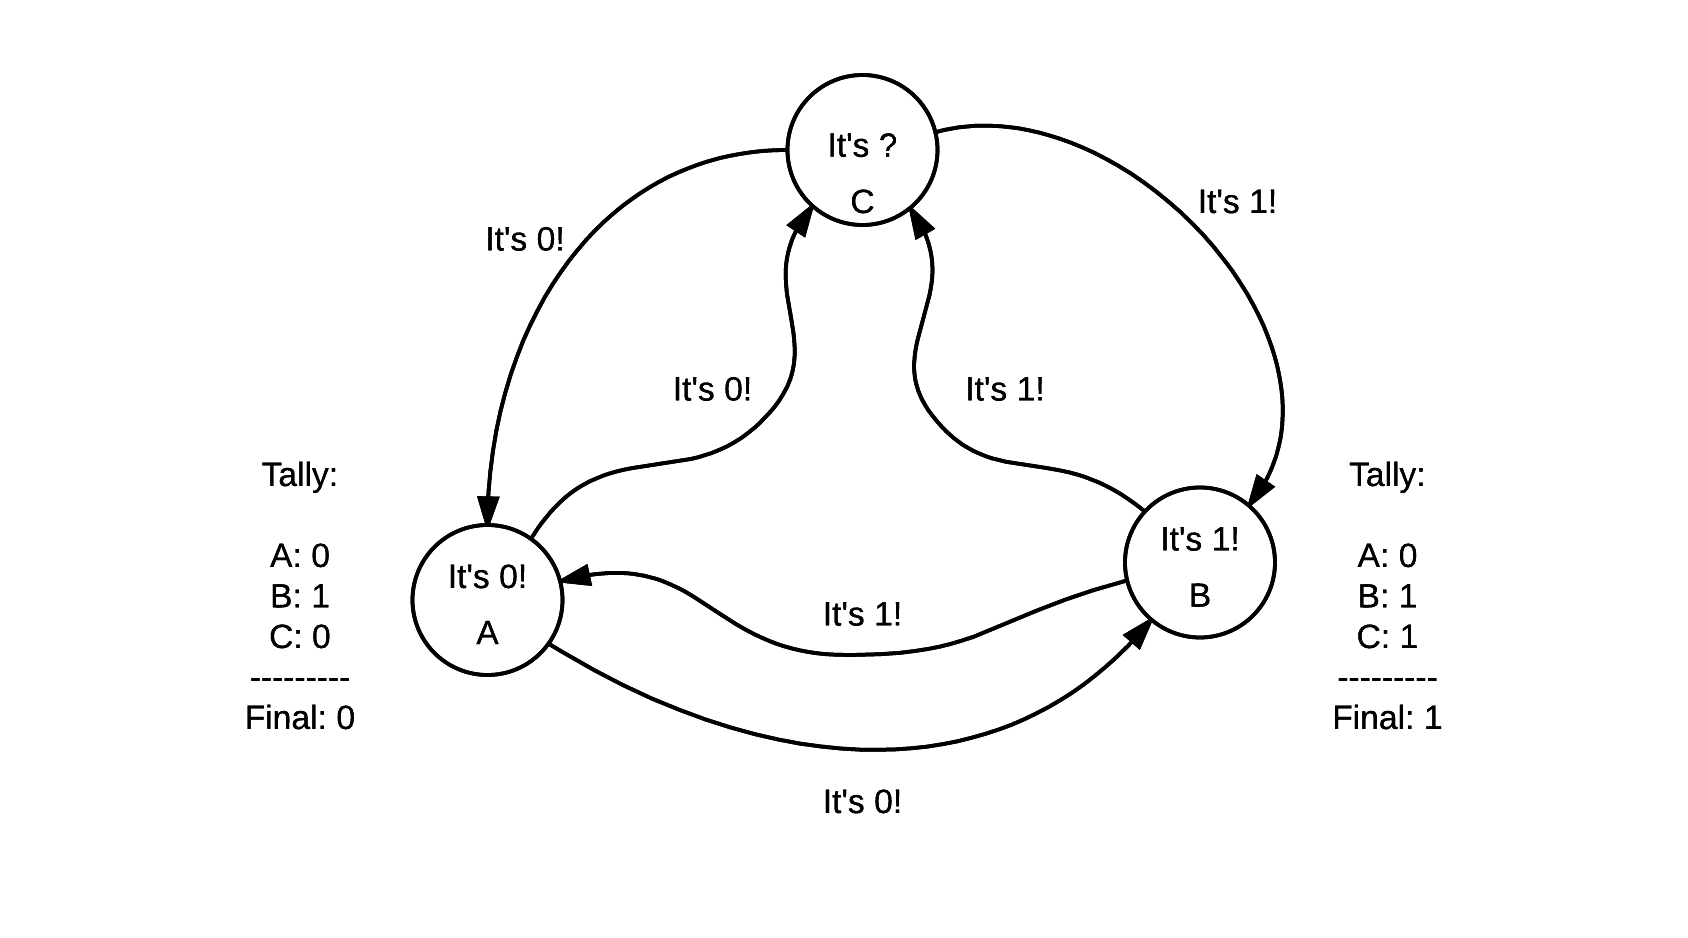
\includegraphics[width=\linewidth,height=\textheight,keepaspectratio]{figures/byzantine.png}
    	\centering
	\label{fig:byzantine}
	\caption[Byzantine nodes tell lies]{
A Byzantine node, C, tells A one thing and B another, causing them to come to different conclusions about the network.
Here, simple majority vote results in a violation of safety due to only a single Byzantine node.}
\end{figure}


In fact, it can be shown that the upper limit on $f$ for Byzantine faults is $f < N/3$ \cite{pease1980reaching}.
Thus, to tolerate a single Byzantine process, we require at least $N=4$. 
Then the faulty process can't split the vote the way it was able to when $N=3$.

In 1999, Castro and Liskov published Practical Byzantine Fault Tolerance \cite{pbft}, or \emph{PBFT}, 
which provided the first optimal Byzantine fault tolerant algorithm in asynchronous networks.
It set a new precedent for the practicality of Byzantine fault tolerance in industrial systems by being capable 
of processing tens of thousands of transactions per second.
Despite this success, Byzantine fault tolerance was still considered expensive and largely unnecessary, 
and the most popular implementation was difficult to build on top of \cite{ppbft}.
Hence, despite a resurgence in academic interest, including numerous improved variations \cite{yin2003separating, kotla2007zyzzyva}
not much progress was made in the way of implementations and deployment.
Furthermore, PBFT provides no guarantees in the face of a complete Byzantine failure, where a third or more of the network is malicious.

\section{The Need For Tendermint}

The success of Bitcoin and its derivatives, especially Ethereum, and their promise of secure, autonomous, distributed, fault-tolerant execution of arbitrary code has caused virtually every major financial institution on the planet to start paying attention to the blockchain phenomenon. 
In particular, there has emerged an understanding of two forms of the technology:
On the one hand are the public blockchains, known affectionately as the Big Bad Public Blockchains or BBPBs, 
whose protocols are dominated by in-built economic incentives bootstrapped by a native currency.
On the other are so called private blockchains, which might more accurately be called ``consortia blockchains'',
and which are effectively improvements on traditional consensus and BFT algorithms through the use of hash trees, digital signatures, 
peer-to-peer networking, and enhanced accountability.

As the infrastructure of our societies continues to decentralize, and as the nature of business becomes more inter-organizational,
there is increasing need for a transparent, accountable, high performance BFT system, which can support applications from finance to domain registration to electronic voting,
and which comes equipped with advanced mechanisms for governance and evolution into the future.
Tendermint is that solution, optimized for consortia, or inter-organizational logic, but flexible enough to accommodate anyone from private enterprise to global currency,
and high-performance enough to compete with the major, non-BFT, consensus solutions available today, such as etcd, consul, and zookeeper, while providing greater resilience, security guarantees, and flexibility to application developers.

A more comprehensive discussion of consensus science and related algorithms is reserved for Chapter \ref{ch:related}

